\documentclass[11pt,a4paper]{article}
\usepackage[utf8]{inputenc}
\usepackage[hmargin=2.0cm,vmargin=2.5cm,bindingoffset=0.5cm]{geometry}
\usepackage{amsfonts}
\usepackage{amsmath,amsthm,amssymb}
\allowdisplaybreaks
\usepackage{hyperref}
\usepackage{graphicx}
\usepackage{tikz}
\usepackage{mathtools}
\DeclarePairedDelimiter\ceil{\lceil}{\rceil}
\DeclarePairedDelimiter\floor{\lfloor}{\rfloor}
%\usepackage{float}
\usepackage{placeins}
\usepackage{diagbox}
\DeclareMathOperator{\Tr}{Tr}
\newtheorem{thm}{Theorem}
\usepackage{subcaption}
%\usepackage{subfigure}
\usepackage[english]{babel}
\author{Mohit}
\title{Does counter-diabatic driving implement adiabaticity by opening energy gap of bare Hamiltonian?  }
\begin{document}
\maketitle
%\tableofcontents
\section{Introduction}

Counter-diabatic Hamiltonian is given as:
\begin{equation}
H_{CD}= H_0 + \dot{\lambda} A_{\lambda} 
\end{equation}

When $\dot{\lambda} \gg 1$, then $H_{CD} \approx \dot{\lambda} A_{\lambda}$

\section{Two level system}
\begin{equation}
H_{LZ}= \Delta \sigma_z + \lambda(t) \sigma_x
\end{equation}

where $\lambda(t)= 2(t-1)/\tau$. Hence, $\dot{\lambda}= 2/\tau$. We are going to start off ground-state of Hamiltonian with $\lambda=-2$ at time $t_i= 1- \tau$ and end our protocol with  $\lambda=2$ at $t_f= 1+ \tau$. Hence, duration of our protocol is $2 \tau$. 

\begin{figure}[!ht]
\begin{center}
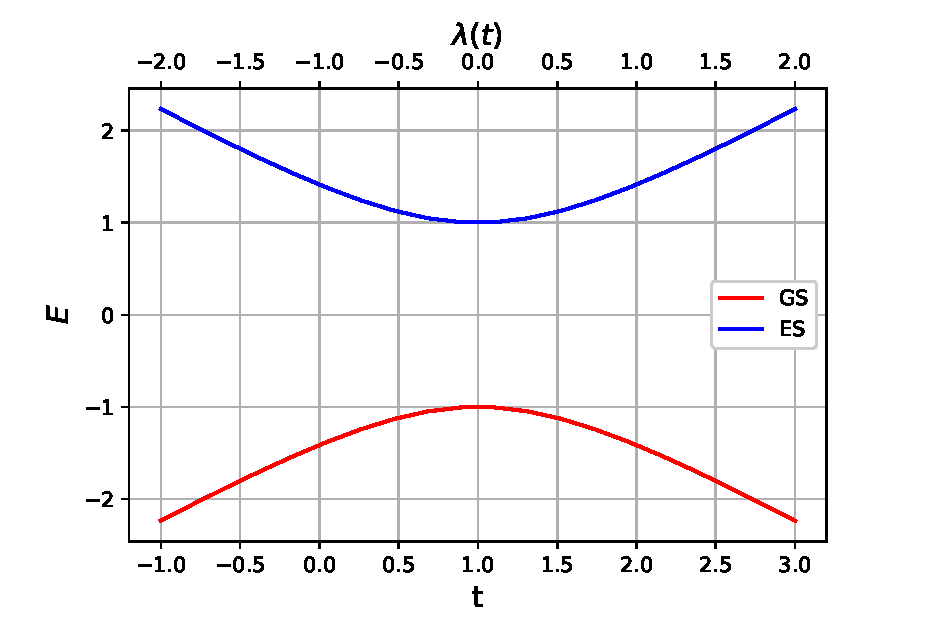
\includegraphics[scale=0.5]{pics/energy_LZ.eps} 
\caption{Avoided level crossing as a function of effective magnetic field with $\Delta=1$ }
\end{center}
\end{figure}

In this case, we know that gauge potential is 
\begin{equation}
A_{\lambda}= \dfrac{\hbar}{2}\dfrac{\Delta }{\Delta^2 + \lambda(t)^2} \sigma^y
\end{equation}
Hence, counter-diabatic Hamiltonian is ($\hbar=1$):
\begin{equation}
H_{CD}= \Delta \sigma_z + \lambda(t) \sigma_x + \dfrac{\dot{\lambda} }{2}\dfrac{\Delta }{\Delta^2 + \lambda(t)^2} \sigma^y
\end{equation}

\begin{figure}[!ht]
\begin{center}
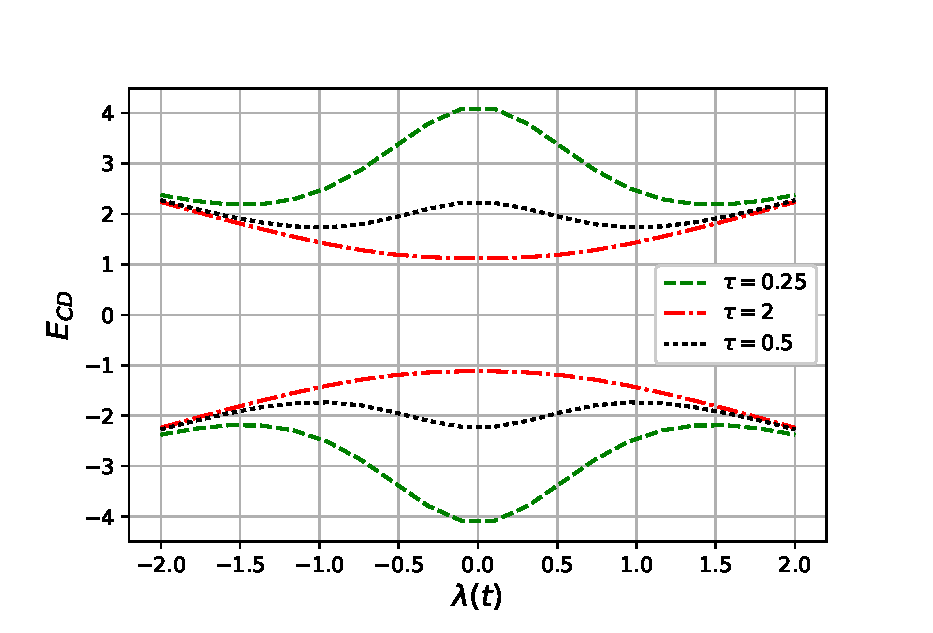
\includegraphics[scale=0.5]{pics/energy_cd_2level_sys.eps} 
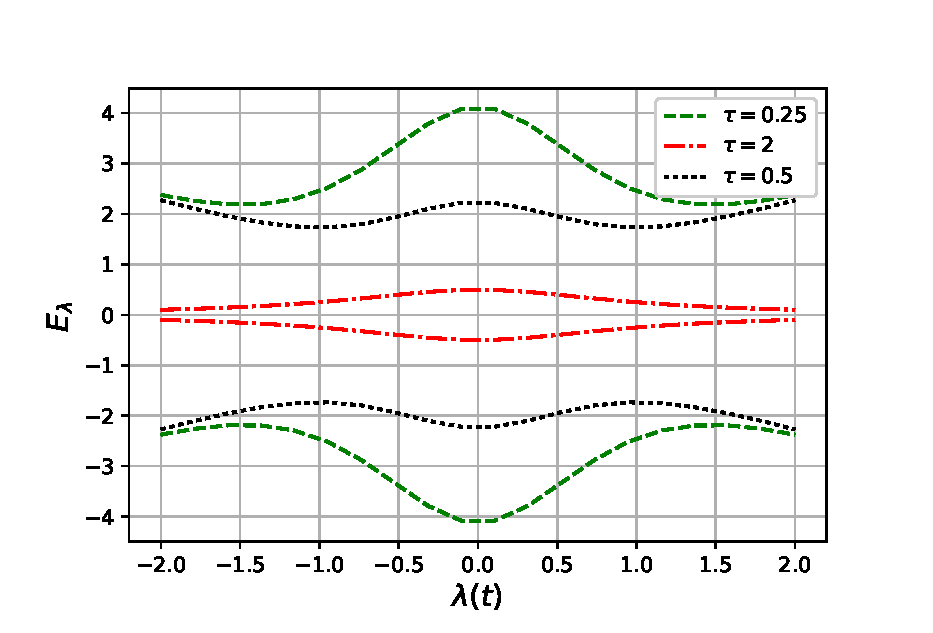
\includegraphics[scale=0.5]{pics/energy_gauge_potn_2level.eps} 
\caption{a) Energy $E_{CD}$ of $H_{CD}$ b) Energy $E_{\lambda}$ of $H= \dot{\lambda}A_{\lambda}$ }
\end{center}
\end{figure}

It seems that energy gap opens up!

\section{Three level system}
\subsection{Spin 1 LZ model}

\begin{equation}
H_{LZ}= \Delta S_z + \lambda S_x
\end{equation}
\begin{equation}
A_{\lambda}= \dfrac{\hbar}{2}\dfrac{\Delta }{\Delta^2 + \lambda(t)^2} S^y
\end{equation}
\subsection{NV model}
\begin{align*}
H_{NV} = \Delta S_z^2 + \lambda   S_x  
\end{align*}
\bibliography{ref} 

\bibliographystyle{unsrt}
%\bibliographystyle{plain}

\end{document}
